\section{Studio prestazionale approfondito dei parametri della variante All-in-One 2.0}
In questo capitolo si andrà a confrontare la proposta finale, ovvero la versione All-in-One 2.0, con la versione base del protocollo GreenWUP con l'obiettivo di studiarne le prestazioni al variare di alcuni parametri come il numero dei nodi, la densità e la fonte di Energy-Harvesting.\\

Sicuramente è interessante vedere come si comportano le due versioni al variare della popolazione della rete e soprattutto non avendo più quell'omogeneità a livello di raccolta di energia, che era invece assunta negli scenari simulativi del precedente capitolo.\\

In particolare, durante i test si continuerà ad usare iaTime di 2, 5, 10, 25, 50 secondi in modo da avere diversi scenari con traffico diverso. Varierà anche, come già detto, il numero di nodi nella rete. Infatti, sono state effettuate simulazioni con 100, 140, 220 nodi in modo da aumentare la densità in rete.\\

Infine, fatto a meno del nodo \textit{sink}, il 50\% dei nodi continuerà ad accumulare energia mediante pannelli solari, mentre l'altra metà dei nodi in rete utilizzerà delle turbine eoliche in modo da avere maggiore eterogeneità tra i componenti della rete.\\

I parametri osservati saranno anche in questo caso la percentuale di pacchetti DATA ricevuti correttamente e il ritardo end-to-end. \\
\newpage

\begin{figure}[h!]
  \begin{subfigure}[t]{0.329\linewidth}
    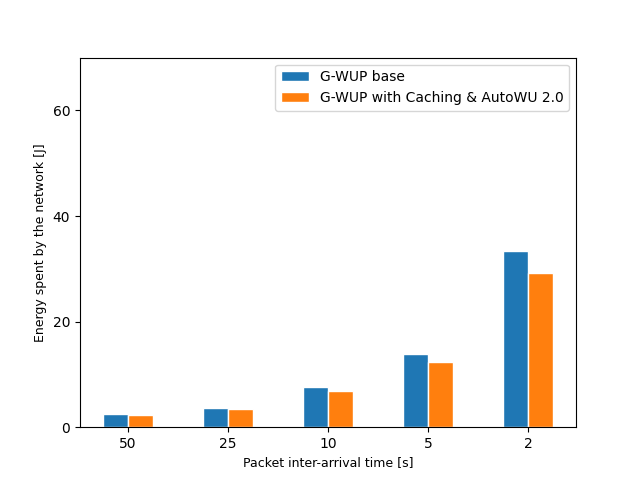
\includegraphics[width=1.13\linewidth]{Contents/Images/graphs/analisi_final2.0/energySpent/energySpent_100.png}
    \caption{100 Nodi}
  \end{subfigure}
  \begin{subfigure}[t]{0.329\linewidth}
    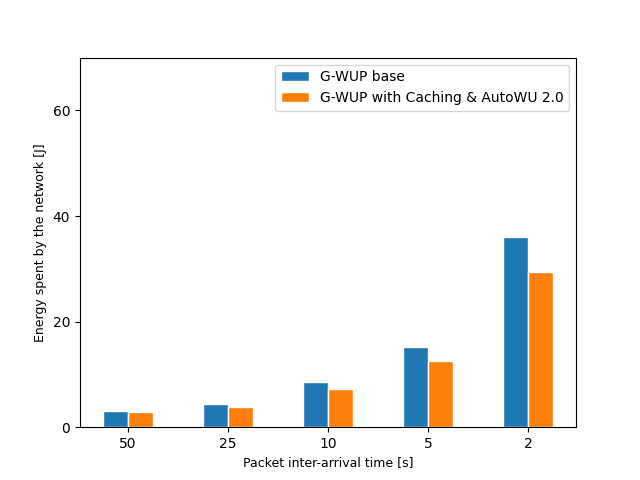
\includegraphics[width=1.13\linewidth]{Contents/Images/graphs/analisi_final2.0/energySpent/energySpent_140.png}
    \caption{140 Nodi}
  \end{subfigure}
  \begin{subfigure}[t]{0.329\linewidth}
    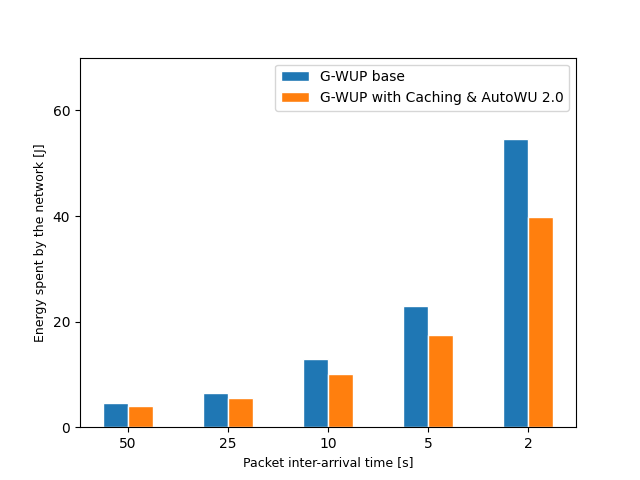
\includegraphics[width=1.13\linewidth]{Contents/Images/graphs/analisi_final2.0/energySpent/energySpent_220.png}
    \caption{220 Nodi}
  \end{subfigure}
  \caption{Risultati ottenuti analizzando l'energia consumata dalla rete}
  \label{fig:analisi_EnergySpent}
\end{figure}

Come mostrato in \textbf{Figura \ref{fig:analisi_EnergySpent}}, la nuova versione di \textit{All-in-One} continua ad ottenere risultati migliori rispetto la versione base di GreenWUP anche cambiando densità e traffico in rete. In particolare dai grafici si evince una crescita dei consumi più lenta rispetto GreenWUP base.\\
Le due proposte, comunque, hanno un comportamento molto simile solo in scenari con poco traffico. Infatti, la differenza di energia aumenta all'aumentare del numero di pacchetti DATA inviati. 

\begin{figure}[h!]
  \begin{subfigure}[t]{0.329\linewidth}
    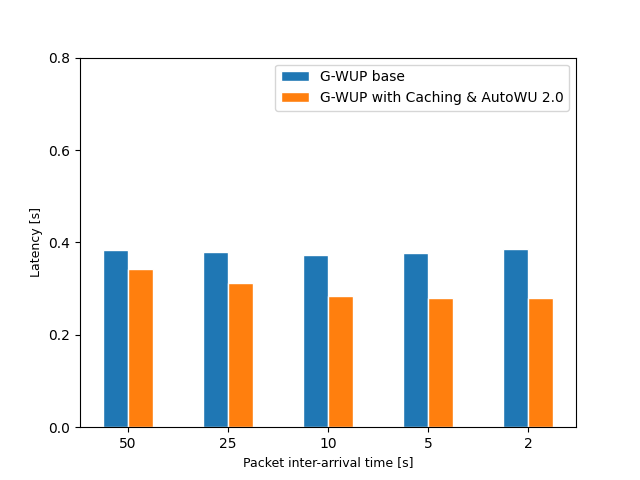
\includegraphics[width=1.13\linewidth]{Contents/Images/graphs/analisi_final2.0/latency/latency_100.png}
    \caption{100 Nodi}
  \end{subfigure}
  \begin{subfigure}[t]{0.329\linewidth}
    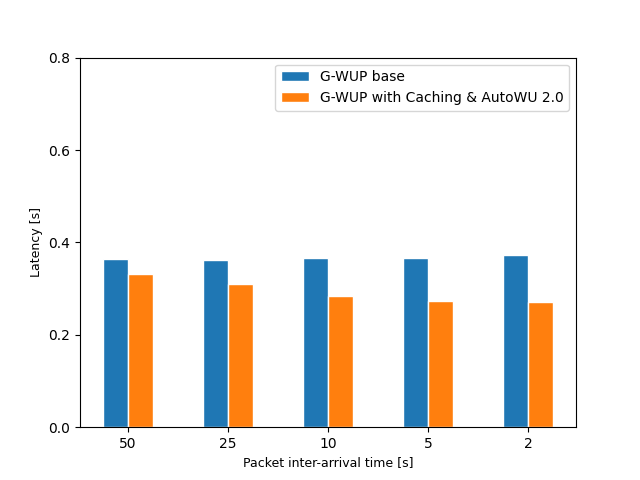
\includegraphics[width=1.13\linewidth]{Contents/Images/graphs/analisi_final2.0/latency/latency_140.png}
    \caption{140 Nodi}
  \end{subfigure}
  \begin{subfigure}[t]{0.329\linewidth}
    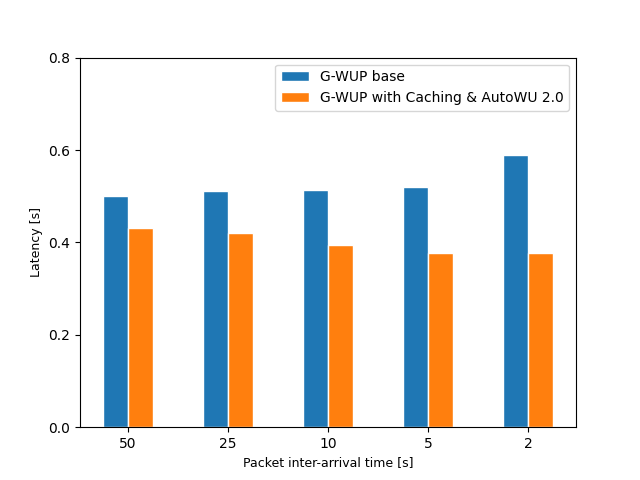
\includegraphics[width=1.13\linewidth]{Contents/Images/graphs/analisi_final2.0/latency/latency_220.png}
    \caption{220 Nodi}
  \end{subfigure}
  \caption{Risultati ottenuti analizzando il ritardo end-to-end}
  \label{fig:analisi_Latency}
\end{figure}

Come mostrato in \textbf{Figura \ref{fig:analisi_Latency}}, anche per il ritardo end-to-end la soluzione proposta risulta essere migliore rispetto alla versione base. \'E possibile notare come all'aumentare del traffico in rete, aldilà della densità della rete, le due versioni di GreenWUP presentino due comportamenti completamente opposti. Infatti per GreenWUP classico il ritardo medio cresce all'aumentare del traffico, mentre per la nuova variante proposta, il ritardo risulta essere minore in scenari in cui il numero di pacchetti DATA è maggiore (proprietà derivante dal caching del next-hop).\\
\newpage

\begin{figure}[h!]
  \begin{subfigure}[t]{0.329\linewidth}
    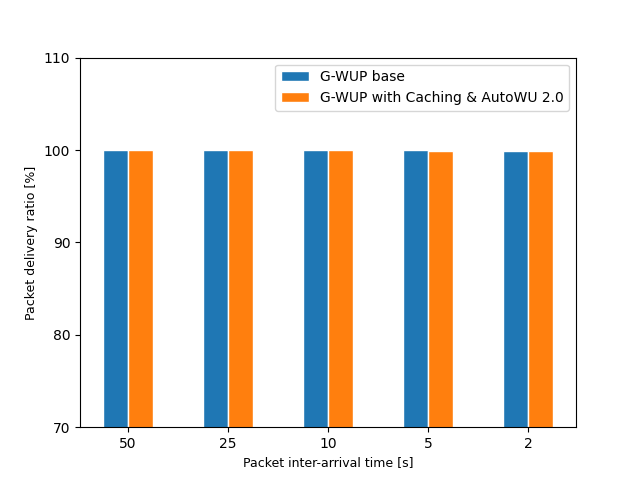
\includegraphics[width=1.13\linewidth]{Contents/Images/graphs/analisi_final2.0/pdr/pdr_100.png}
    \caption{100 Nodi}
  \end{subfigure}
  \begin{subfigure}[t]{0.329\linewidth}
    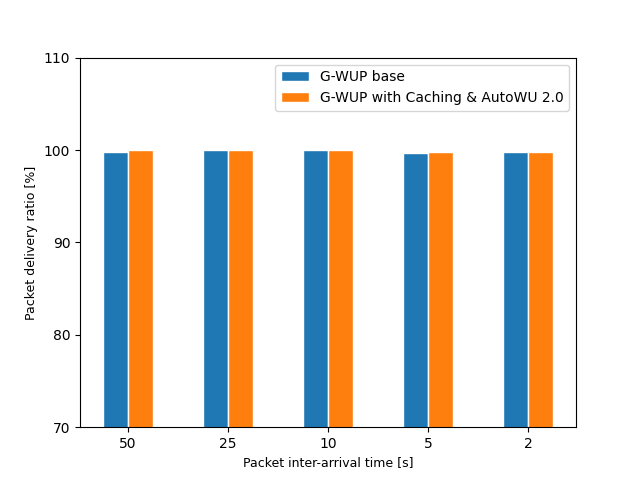
\includegraphics[width=1.13\linewidth]{Contents/Images/graphs/analisi_final2.0/pdr/pdr_140.png}
    \caption{140 Nodi}
  \end{subfigure}
  \begin{subfigure}[t]{0.329\linewidth}
    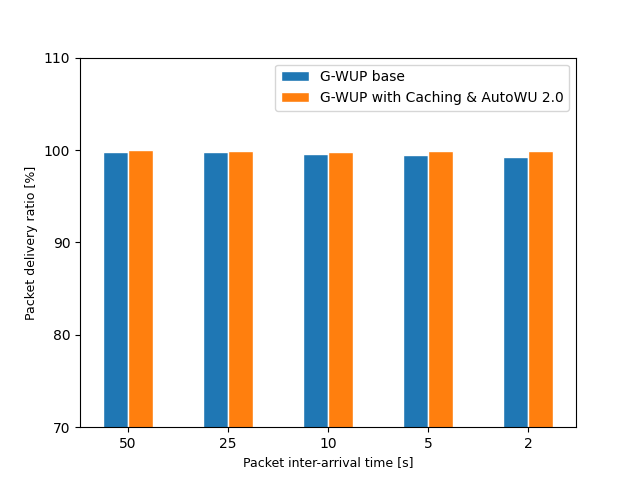
\includegraphics[width=1.13\linewidth]{Contents/Images/graphs/analisi_final2.0/pdr/pdr_220.png}
    \caption{220 Nodi}
  \end{subfigure}
  \caption{Risultati ottenuti analizzando i pacchetti ricevuti correttamente}
  \label{fig:analisi_pdr}
\end{figure}

Come mostrato in \textbf{Figura \ref{fig:analisi_pdr}}, entrambe le soluzioni forniscono sempre una percentuale di pacchetti DATA correttamente ricevuti di almeno il 99\%.\\
Infatti è possibile notare come i risultati siano pressoché identici per le due soluzioni, fatta eccezione per la configurazione con 220 Nodi in cui è possibile vedere un leggero miglioramento rispetto la versione base di GreenWUP nella variante proposta.\\
Sicuramente la migliore gestione dei ritardi e soprattutto dell'energia consumata dalla rete ha fatto il modo di ridurre il numero di pacchetti persi rendendo, di fatto, la variante proposta una valida alternativa alla versione base di GreenWUP.